\documentclass{article}

%\usepackage[spanish]{babel}

\usepackage[utf8]{inputenc}

\usepackage{graphicx}

\title{Ecuaciones en diferencias}


\author{Mauricio Islas Gómez}

\begin{document}

\maketitle

\section{Ecuaciones de primer grado}

\subsection{Ecuaciones lineales}

Una ecuacion lineal en diferencias de primer grado tiene la forma $x_{n+1}=ax_{n}$ donde $a$ es una constante.

La fórmula para resolver ecuaciones lineales es:
\begin{equation}
  \label{eq:2}
  x_n=a^nx_0
\end{equation}.

Por ejemplo, si iniciamos una inversion con 1000 pesos con un inreres mensual de 1\%, obtenemos lo siguiente

\begin{center}
  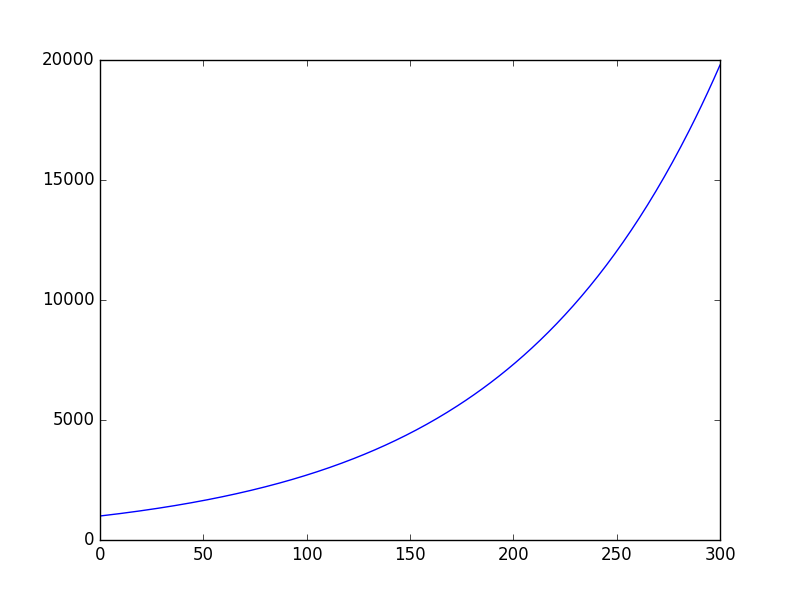
\includegraphics[width=8cm]{inversion.png}
\end{center}
\subsection{Ecuaciones Afines}

Una ecuacion afin en diferencias de primer grado tiene la forma $x_{n+1}=ax_{n}$ donde $a$ es una constante.

\begin{equation}
  \label{eq:1}
  x_n=a^n(x_0-\alpha)+\alpha
\end{equation}

donde $\alpha=\frac{b}{1-a}$.

Para deducir ésta formula usamos $$\sum_{i=0}^{n-1}a^i=\frac{a^n-1}{a-1}$$.

\section{Ecuaciones de segundo grado}

El método para resolver estas ecuaciones está inspirado en la formula (\ref{eq:2}).

% Una ecuacion lineal en diferencias de primer grado tiene la forma $x_{n+1}=ax_{n}$ donde $a$ es una constante.


\end{document}
